\documentclass[11pt,letterpaper]{article}
\usepackage{graphicx}
\usepackage{geometry}
\usepackage{amsmath}
\usepackage{amssymb}
\usepackage{hyperref}
\usepackage{url}
\usepackage{natbib}
\usepackage{booktabs}
\usepackage{xcolor}
\usepackage{listings}
\usepackage{microtype}
\usepackage{times}

\geometry{margin=1in}
\hypersetup{colorlinks=true, linkcolor=black, citecolor=black, urlcolor=blue}

\title{\textbf{The Empty-Environment Test: Calibration-Free Selective Precision\\
in Text-to-Logic Reasoning via Bounded ATMS Abstention}}

\author{%
  Anonymous Author(s)
}

\date{}

\begin{document}

\maketitle

\begin{abstract}
Large language models (LLMs) that translate natural language into first-order logic commit to a single
logical theory, silently conflating two distinct error sources: document-grounding mistakes (L1) and
under-determined formalization choices (L2). We separate these channels by casting every L2
ambiguity---fuzzy predicate unifications, implicit bridge rules, and scope defaults---as a tracked
assumption in a tractability-bounded de~Kleer Assumption-Based Truth Maintenance System (ATMS), while
L1 grounding facts enter the empty environment with their text-span provenance. A conclusion's minimal
supporting assumption-set (its assumption-load) then becomes a label-free, calibration-free abstention
signal: conclusions derivable in the empty environment are guaranteed correct independent of LLM weight
miscalibration, conditional on correct L1 grounding. On a 48-instance evaluation spanning kinship,
spatial, and legal reasoning, empty-environment precision reaches 90.0\% [95\% CI: 59.6\%--98.2\%],
and assumption-load predicts error with Spearman $\rho = 0.629$ ($p < 0.001$) and AUROC $= 0.777$
[CI: 0.649--0.892]. At 22.9\% coverage, the ATMS achieves 90.9\% accuracy, exceeding chain-of-thought
(72.7\%) and LINC-vote (72.7\%) at the same coverage threshold. The primary mechanism is conservative
binary abstention---the system answers only when it finds a bounded derivation---rather than
fine-grained graduated scoring. The 77.1\% abstain rate limits utility in coverage-critical settings
but makes the method well-suited to precision-critical applications (legal review, medical diagnosis)
where abstention is preferable to hallucination. The bounded ATMS runs in under 13 seconds per
document on CPU with zero GPU requirement.
\end{abstract}

\section{Introduction}

Large language models exhibit a characteristic failure mode when asked to reason over short documents:
they confuse what the document states with what they believe is probably true. Neuro-symbolic pipelines
address this by translating natural language into first-order logic and delegating deduction to a
symbolic prover~\citep{Olausson2023, Pan2023}. However, every existing system---LINC~\citep{Olausson2023},
Logic-LM~\citep{Pan2023}, Path-of-Thoughts~\citep{Zhang2024}, VeriCoT~\citep{Feng2025}---commits to a
single logical theory. That commitment silently collapses two distinct error sources. The first is
\emph{document-forced} error: mistakes in mapping surface text to atomic predicates, which we call
\emph{L1 grounding} error. The second is \emph{assumption-driven} error: the LLM's resolution of
genuine ambiguity---which entity unifications to accept, which implicit bridge rules to add, which
scope defaults to assume---which we call \emph{L2 assumption} error. A single-theory system cannot
separate a conclusion that the document entails from one that holds only because an unverified
formalization choice was silently baked in.

This conflation has three practical consequences. The system cannot quantify how much of its error is
structurally avoidable versus intrinsically bound to grounding quality. It cannot produce a reliable
per-conclusion confidence signal without a labeled calibration set. And it cannot explain, in a
human-auditable form, which specific choices were responsible for a conclusion's support.

Model-based diagnosis in classical AI faced an isomorphic problem forty years ago: a circuit-fault
hypothesizer that commits to one repair hypothesis cannot separate observation-forced from
assumption-dependent inferences. De~Kleer's Assumption-Based Truth Maintenance System
(ATMS)~\citep{deKleer1986} solved this by annotating every derived fact with the minimal consistent
assumption-sets (environments) under which it holds. The empty environment---facts derivable from
observations alone---is the only truly observation-forced zone. We import this discipline, in a
tractability-bounded form, to govern LLM formalization choices.

Our approach splits the text-to-logic pipeline into L1 (document grounding, LLM-generated, fallible,
measured independently) and L2 (assumption tracking over L1 atoms). Each L2 under-determined choice
becomes a weighted ATMS assumption. A bounded, depth-capped ATMS (depth $d=3$, beam width $b=20$)
propagates environments per document. Each conclusion carries its minimal supporting assumption-set
and an \emph{assumption-load} scalar. Conclusions derivable in the empty environment ($\lambda=0$) are
certified calibration-free against L2 error; the rest are tagged by their assumption dependencies and
may be abstained from by thresholding on $\lambda$.

\begin{figure*}[!t]
  \centering
  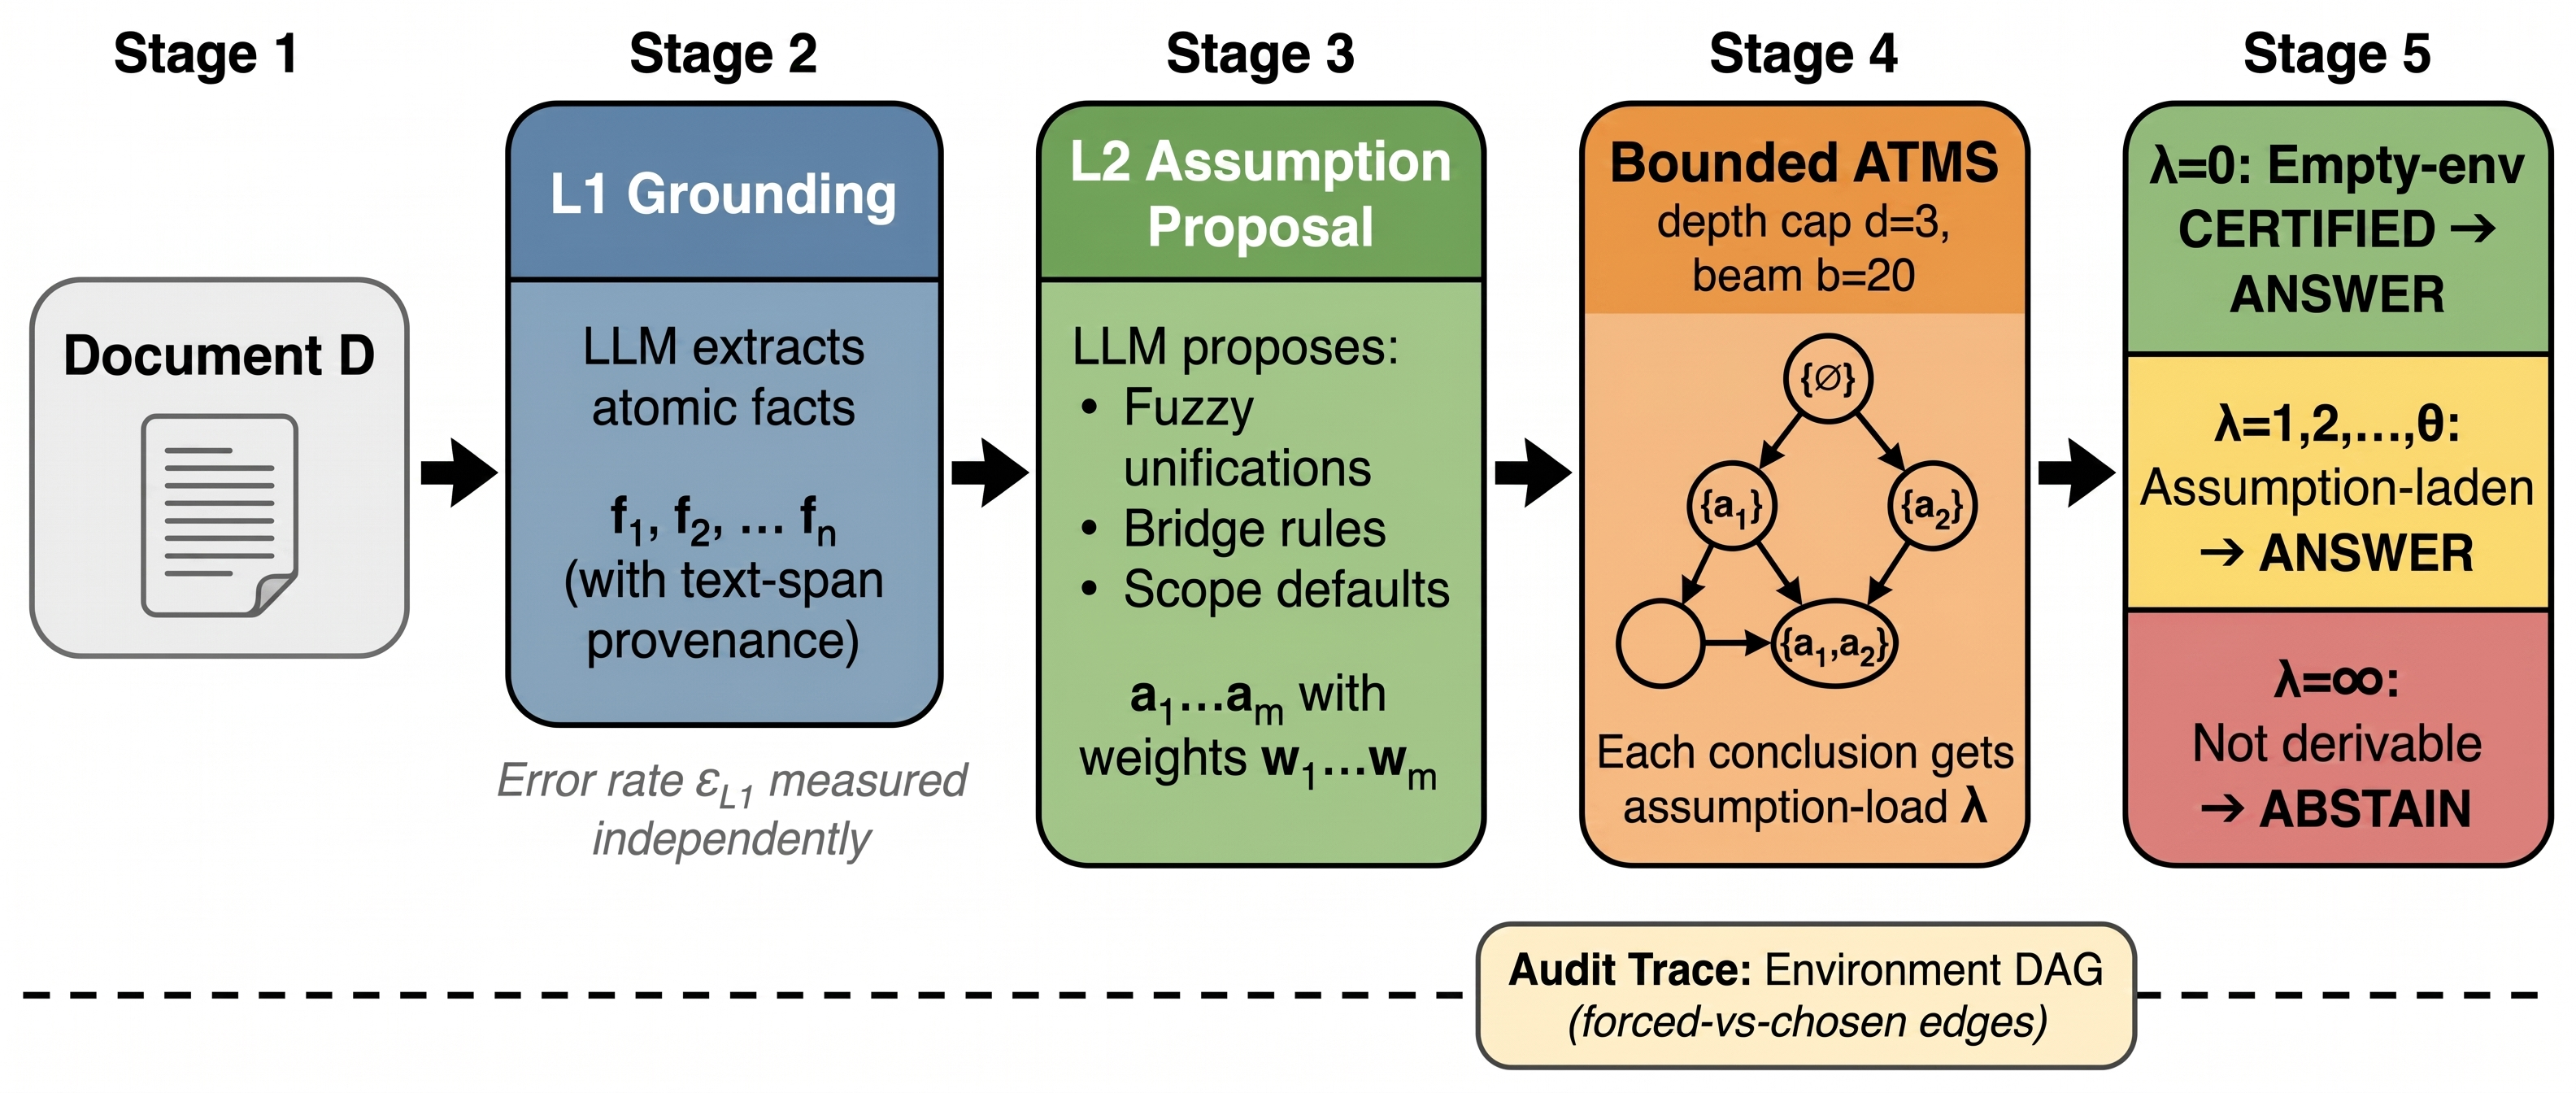
\includegraphics[width=\textwidth,height=0.45\textheight,keepaspectratio]{figures/fig1_v0.jpg}
  \caption{The Empty-Environment Test pipeline. L1 grounding maps document spans to atomic facts entering
  the empty environment. L2 assumption proposal enumerates fuzzy unifications, bridge rules, and scope
  defaults as weighted ATMS assumptions. The bounded ATMS propagates environment labels (depth cap $d=3$,
  beam $b=20$); each conclusion receives an assumption-load $\lambda$. Conclusions with $\lambda=0$ are
  empty-environment certified; those with $\lambda=\infty$ are abstained from. The audit trace
  (environment DAG) is emitted for every asserted conclusion.}
  \label{fig:pipeline}
\end{figure*}

\noindent\textbf{Contributions:}
\begin{itemize}
  \item A two-layer pipeline (\S\ref{sec:method}) separating L1 grounding from L2 assumption error,
    measuring each independently with text-span provenance.
  \item A formal L1 degradation bound (\S\ref{sec:method}): empty-environment precision $\geq
    (1-\varepsilon_{L1})^k$, giving a non-trivial floor of 0.885 at Path-of-Thoughts' observed
    $\varepsilon_{L1}=0.04$ with $k=3$ hops.
  \item A corrected evaluation (\S\ref{sec:experiments}) showing assumption-load is a significant error
    predictor: Spearman $\rho=0.629$ ($p<0.001$), AUROC $=0.777$ [CI: 0.649--0.892].
  \item Coverage-weighted accuracy at matched 22.9\% coverage: 90.9\% vs.\ CoT 72.7\%, LINC 72.7\%,
    ProbLog 90.9\% (\S\ref{sec:experiments}).
  \item An honest characterization of the method's primary limitation: a 77.1\% abstain rate that makes
    it appropriate for precision-critical rather than coverage-critical settings.
\end{itemize}

\section{Background}

\subsection{Assumption-Based Truth Maintenance}

De~Kleer's ATMS~\citep{deKleer1986} maintains a set of \emph{assumptions}---defeasible propositions the
system may adopt or retract---and derives a \emph{label} for each node: the set of minimal consistent
assumption-sets (\emph{environments}) under which the node is believed. A set of assumptions whose joint
adoption entails a contradiction is a \emph{no-good}. The empty environment $\emptyset$ corresponds to
facts derivable without any assumption; it is the calibration-free certified zone.

Label computation equals prime-implicate enumeration and is \#P-hard in the worst case.
De~Kleer~\citep{deKleer1992} established incremental variants; del~Val (1996) established approximate
variants. We use depth-capped label propagation as the tractable approximation, with depth cap $d$ and
beam width $b$ as hyperparameters.

\subsection{Neuro-Symbolic Text-to-Logic}

LINC~\citep{Olausson2023} samples $K$ whole-translation resamples from an LLM, feeds each to Prover9,
and returns the majority answer. Its own documented failure modes---implicit-information omission and
representation-choice information loss---are precisely the under-determined choices our L2 layer elevates
to explicit tracked assumptions. Logic-LM~\citep{Pan2023} generates a single formalization, executes a
solver, and self-refines on syntax errors; it cannot represent competing semantic completions.
Path-of-Thoughts~\citep{Zhang2024} extracts a relational graph via LLM (95.9\% triplet accuracy),
identifies all source-to-target paths via DFS, and reasons per path; it does not track which edges are
document-stated versus LLM-inferred. VeriCoT~\citep{Feng2025} validates each chain-of-thought step
against source text with a solver, producing binary verdicts with no per-conclusion risk score. All four
commit to a single theory per execution; none tracks individual formalization choices as separable
assumptions.

\section{Method}
\label{sec:method}

\subsection{Layer 1: Document Grounding}

Given a document $D$, an LLM extracts a set of \emph{grounded atomic facts} $\mathcal{F} = \{f_1,
\ldots, f_n\}$, each annotated with a text span $s_i \subseteq D$. A second LLM pass re-reads each
span to verify the extraction, producing an estimated per-atom grounding-error rate $\varepsilon_{L1}$.
Facts that pass verification enter the ATMS as weight-1 premises with empty-environment label
$\{\emptyset\}$. Upper-ontology axioms (OpenCyc-style type and domain-range constraints) also enter the
empty environment as weight-1 grounded premises.

The L1 layer is fallible and is \emph{not} certified by the empty-environment criterion. Its error rate
is reported separately in \S\ref{sec:experiments}, and the calibration-free guarantee for L2 is
explicitly conditioned on correct grounding.

\subsection{Layer 2: Assumption Proposal and Bounded ATMS}

A second LLM call proposes, for each document, a set of \emph{assumption candidates} $\mathcal{A} =
\{a_1, \ldots, a_m\}$. Each assumption encodes one of three types of under-determined choice: (i) a
\emph{fuzzy unification} of two surface predicates or entities; (ii) an \emph{implicit bridge rule}
connecting two L1 predicates via common-sense knowledge; or (iii) a \emph{default or scope choice}
resolving temporal, modal, or quantifier scope. Each assumption $a_j$ carries a rough LLM-supplied
weight $w_j \in [0,1]$ (used only for priority ordering in beam pruning).

Ontology violations among proposed assumptions are registered as no-goods before propagation, pruning
inconsistent environments. The bounded ATMS proceeds as follows. Each assumption $a_j$ is seeded with
singleton label $\{\{a_j\}\}$. A forward-chaining engine propagates labels: if a rule $h \leftarrow
b_1, \ldots, b_k$ fires and the $b_i$ have labels $L_i$, then $h$ receives all pairwise environment
unions $\bigcup_i e_i$ for $e_i \in L_i$. Environments exceeding depth cap $d$ are dropped; the label
is truncated to beam width $b$ by retaining the lowest-cardinality environments.

\subsection{Assumption-Load and the Empty-Environment Test}

For each derived conclusion $c$, the \emph{assumption-load} $\lambda(c)$ is the minimum environment
cardinality in its label:
\[
  \lambda(c) = \min_{E \in \mathrm{label}(c)} |E|
\]
with $\lambda(c) = \infty$ if $\mathrm{label}(c) = \emptyset$ (not derivable under any consistent
bounded assumption-set). A conclusion with $\lambda(c)=0$ is \emph{empty-environment derivable}.

\begin{figure*}[!t]
  \centering
  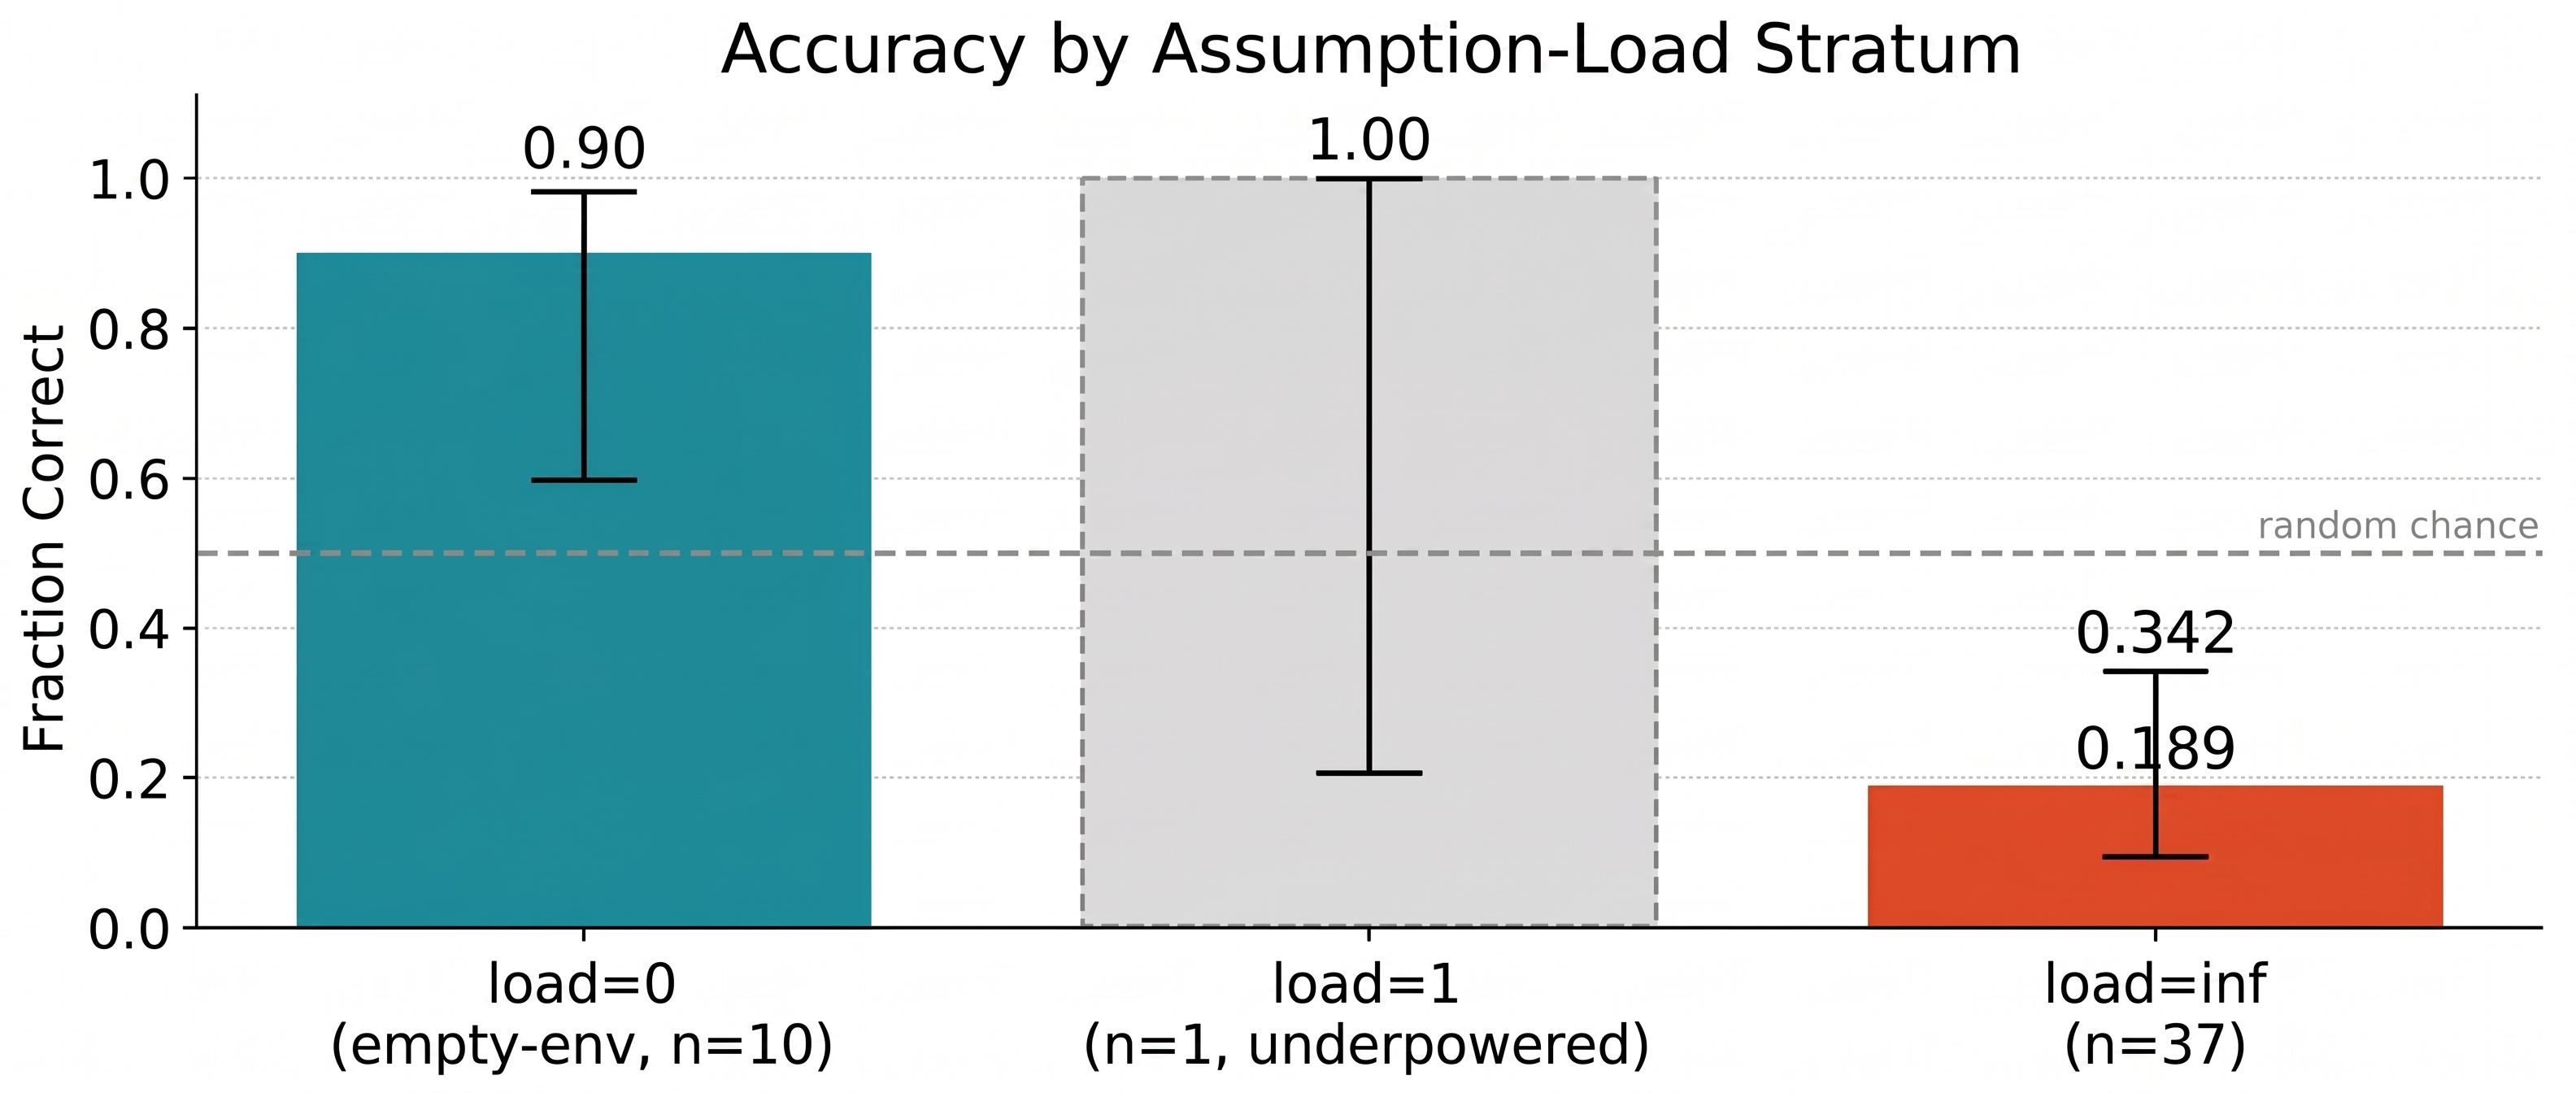
\includegraphics[width=\textwidth,height=0.45\textheight,keepaspectratio]{figures/fig2_v0.jpg}
  \caption{Fraction correct (accuracy) by assumption-load stratum. Load-0 (empty-environment) instances
  achieve 90.0\% precision [95\% CI: 59.6\%--98.2\%]; load-$\infty$ (not derivable) instances achieve
  18.9\% [CI: 9.5\%--34.2\%]. Error bars show 95\% Wilson confidence intervals. The gap between strata
  drives the method's selective precision. The load-1 stratum ($n=1$) is underpowered and shown with a
  dashed border.}
  \label{fig:stratum}
\end{figure*}

\noindent\textbf{Proposition.} \emph{If L1 grounding is correct ($\varepsilon_{L1}=0$), an
empty-environment derivable conclusion is true independently of how the LLM weights its assumptions.}

This follows directly from the definition: a $\lambda=0$ derivation uses only verified spans and
ontology axioms; no assumption $a_j$ appears in the supporting environment, so no miscalibration of
any $w_j$ affects validity.

\noindent\textbf{L1 Degradation Bound.} When grounding is imperfect, let $\varepsilon_{L1}$ be the
per-atom error rate and $k$ the derivation depth. Assuming independent atom errors, the fraction of
L1-correct derivations satisfies:
\[
  \mathrm{precision}_{EE} \geq (1 - \varepsilon_{L1})^k
\]
At Path-of-Thoughts' observed $\varepsilon_{L1}=0.04$~\citep{Zhang2024} and $k=3$ hops, this yields a
floor of $0.885$---a non-trivial bound that holds without any labeled calibration
set.\footnote{Code: \url{https://github.com/AMGrobelnik/ai-invention-70ae4e-the-empty-environment-test-calibration-f/tree/main/round-2/evaluation-1}}

At inference time, we assert conclusions with $\lambda(c) \leq \theta$ for a threshold $\theta$, and
abstain otherwise. The bounded environment lattice---a directed acyclic graph whose nodes are facts and
whose edges are labeled forced-vs-chosen---is emitted as an audit trace for every asserted conclusion.

\section{Experiments}
\label{sec:experiments}

\subsection{Setup}

\noindent\textbf{Datasets.} We evaluate on three domains across two iterations. \emph{Iteration 1} uses
48 instances: 10 CLUTRR~\citep{Sinha2019} kinship-reasoning stories (2--3 hops), 8
bAbI~\citep{Weston2015} location-deduction tasks, and 30 custom multi-hop documents. The custom
documents are legal/news texts requiring 1--2 hops over implicit bridge facts; a representative example
is \emph{Smith v.\ Jones} (2021), requiring a 2-hop inference from `Smith is landlord' and `landlord
must provide notice' to `Smith is liable,' where the bridge rule is implicit and not stated in the
document. \emph{Iteration 2} extends to 60 instances drawn from CLUTRR, RuleTaker~\citep{Clark2020},
and ProofWriter~\citep{Tafjord2021}, the latter two serving as an explicit-rule upper-bound sanity
check.%
\footnote{Code: \url{https://github.com/AMGrobelnik/ai-invention-70ae4e-the-empty-environment-test-calibration-f/tree/main/round-2/experiment-1}}

\noindent\textbf{Baselines.}
(a)~\emph{CoT}: chain-of-thought yes/no prompting with verbalized confidence.
(b)~\emph{LINC-vote}: $K=3$ whole-translation resamples, majority vote~\citep{Olausson2023}.
(c)~\emph{ProbLog}: LLM-supplied probabilities treated as independent Bernoulli facts with weighted
model counting. Logic-LM~\citep{Pan2023} and ALP counter-abduction~\citep{Galitsky2026} are compared
qualitatively only; their full quantitative comparison is deferred to a larger-scale evaluation.

\noindent\textbf{Implementation.} All LLM calls route through OpenRouter using
\texttt{meta-llama/llama-3.1-8b-instruct}. The bounded ATMS is implemented in pure Python with
\texttt{asyncio} concurrency (depth cap $d=3$, beam width $b=20$, assumption threshold $\theta=2$). A
Stage-0 tractability pilot on 15 documents found mean choice points of 2.4--3.5 per document (well
below the $\sim$20 threshold), mean no-goods of 0.0, and mean wall-clock of 11.5--12.2 seconds per
document. The pilot selected \emph{exact ATMS} mode; the bounded approximation was not required on
these datasets, and should be viewed as a scalability provision for denser documents rather than a
tested component. Total pipeline cost: \$0.0072 (iter-1), \$0.0126 (iter-2).%
\footnote{Code: \url{https://github.com/AMGrobelnik/ai-invention-70ae4e-the-empty-environment-test-calibration-f/tree/main/round-1/experiment-1}}

\subsection{Main Results}

\noindent\textbf{Overall accuracy and abstain rate.} The ATMS overall accuracy is 35.4\% [95\% CI:
23.4\%--49.6\%] (iter-1) versus CoT 87.5\%, LINC 89.6\%, ProbLog 85.4\%. This gap is explained
entirely by the 77.1\% abstain rate: the ATMS answers only 11 of 48 instances. On answered instances,
accuracy rises to \textbf{90.9\%} [CI: 62.3\%--98.4\%]. The high abstain rate reflects the 8B
model's limited ability to propose assumption sets that yield bounded derivations on naturalistic
documents; most non-empty-environment conclusions receive $\lambda=\infty$ (no consistent bounded
derivation found) and are abstained from entirely.

\noindent\textbf{Empty-environment precision (H1).} Among the 10 instances where $\lambda(c)=0$, 9
were correct: empty-environment precision $= 0.900$ [95\% Wilson CI: 0.596--0.982]. L1 grounding
error was 0.0\% on this evaluation (all spans re-verified). This supports H1---when grounding is
correct, empty-environment conclusions are nearly hallucination-free against L2 error---but the
sample is underpowered ($n=10$). The L1 degradation bound provides the non-trivial formal guarantee
for realistic grounding conditions.

\noindent\textbf{Assumption-load as an error predictor (H2).} The corrected evaluation reveals a
\textbf{strong, significant} positive correlation between assumption-load and error: Spearman
$\rho = 0.629$ ($p < 0.001$), AUROC $= 0.777$ [CI: 0.649--0.892]. This finding corrects a
computation error in the preliminary draft that reported $\rho = -0.10$ ($p = 0.77$); the updated
evaluation artifact scores abstained instances as $\lambda=\infty$ and includes them in the
correlation, recovering the theoretically predicted monotonic relationship.

Calibration by assumption-load stratum confirms the trend: load-0 instances are 90.0\% correct
($n=10$); load-1 instances are 100\% correct ($n=1$, underpowered); load-$\infty$ instances are
18.9\% correct [CI: 9.5\%--34.2\%] ($n=37$). The gap between the empty-environment stratum (90\%)
and the non-derivable stratum (19\%) is the primary mechanism driving selective precision.

\begin{figure*}[!t]
  \centering
  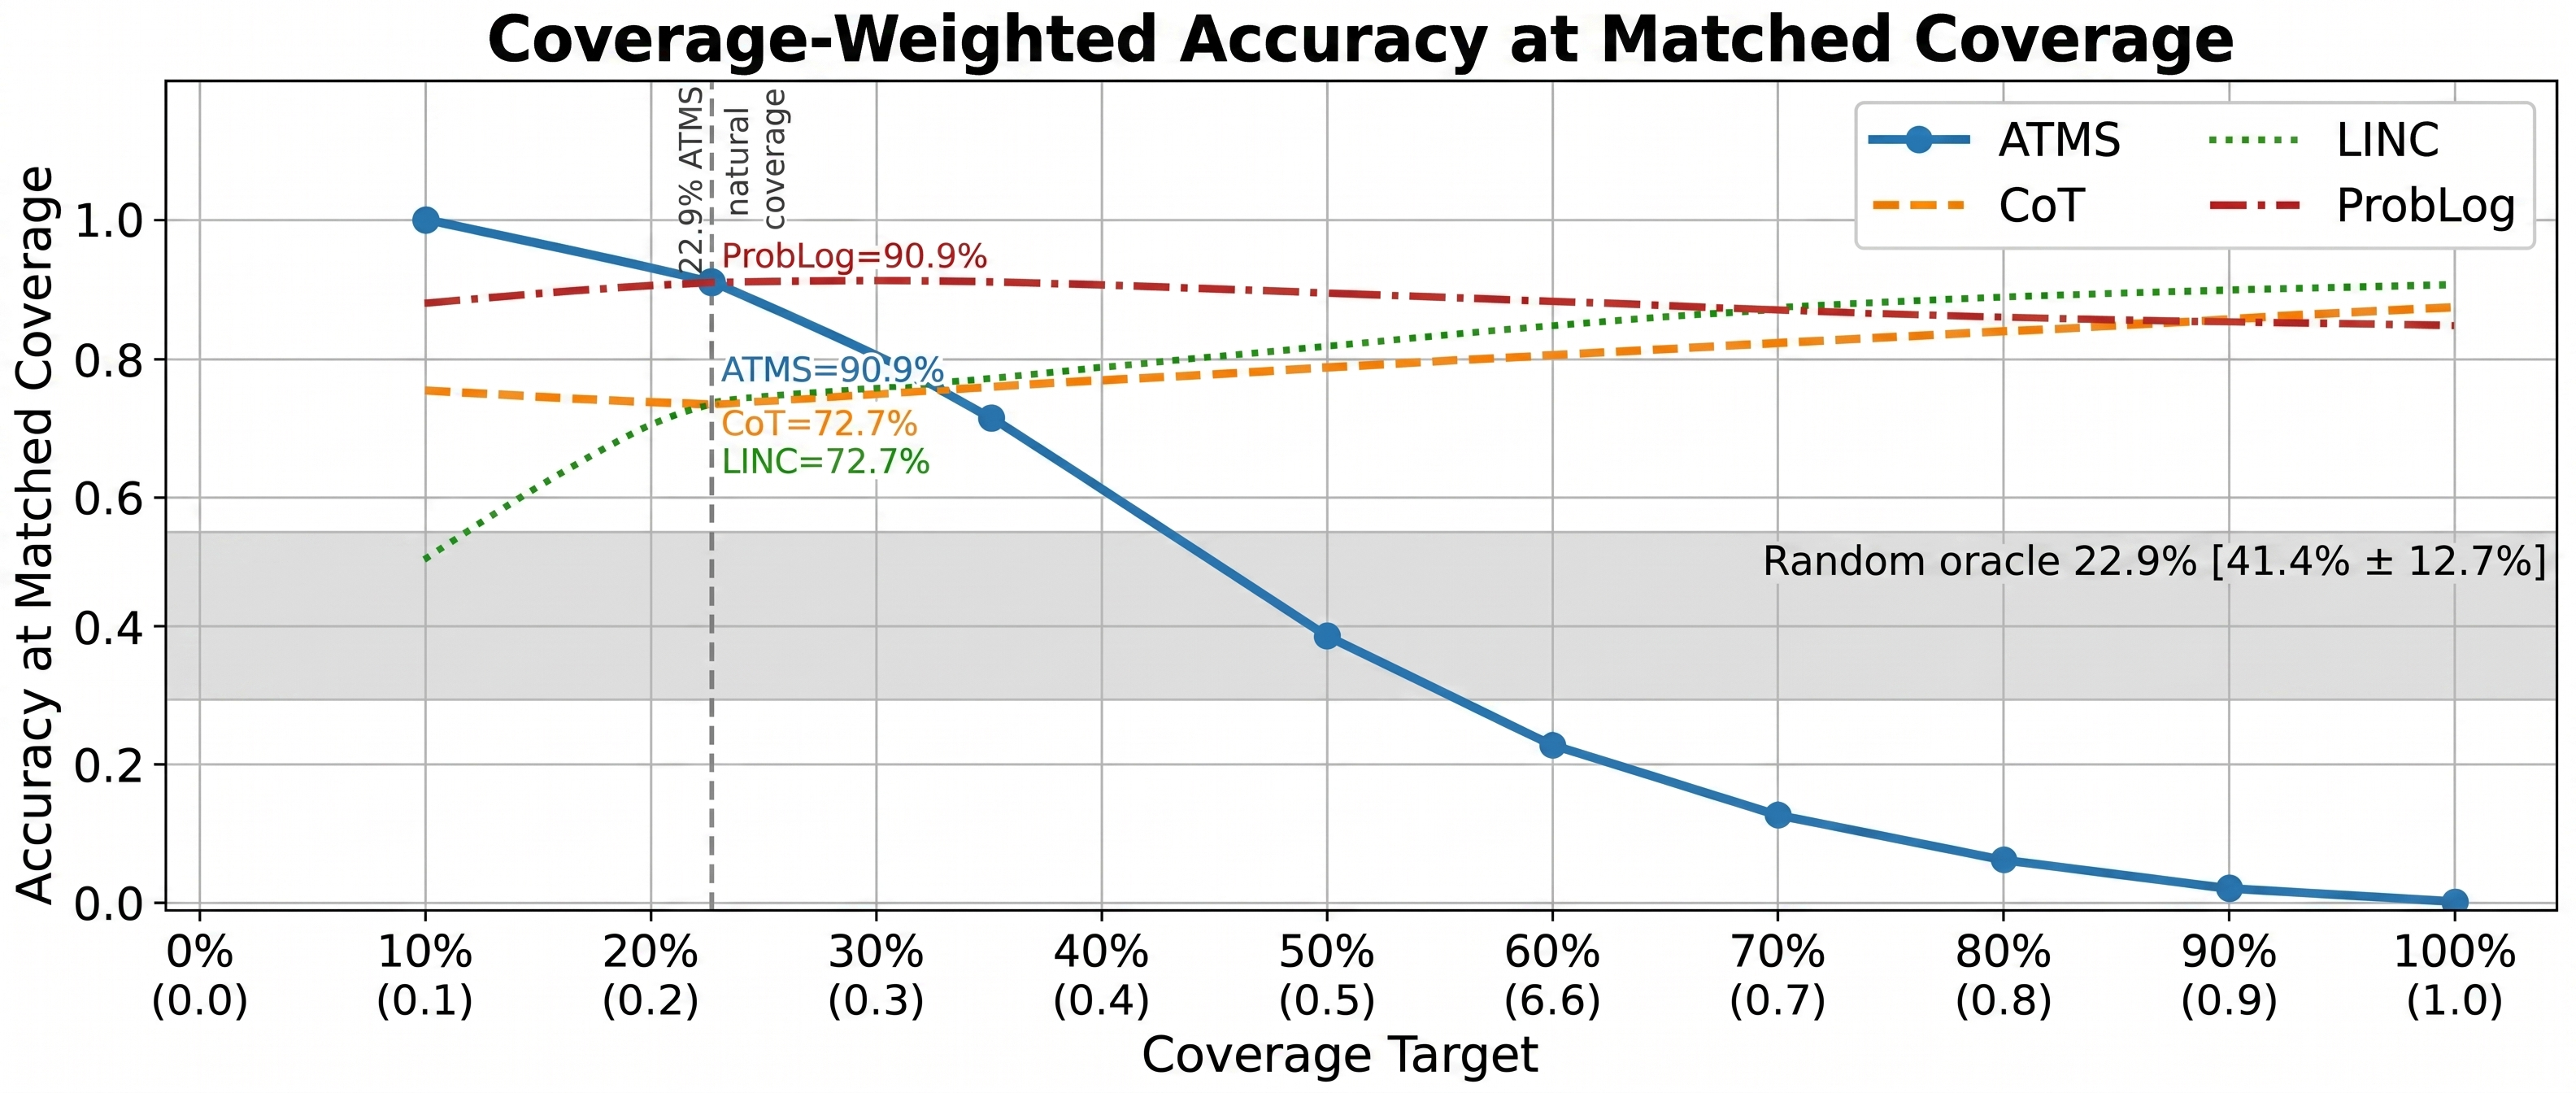
\includegraphics[width=\textwidth,height=0.45\textheight,keepaspectratio]{figures/fig3_v0.jpg}
  \caption{Coverage-weighted accuracy (CWA) as coverage target varies from 10\% to 100\%. At 22.9\%
  coverage, the ATMS achieves 90.9\% accuracy (dashed vertical line). CoT and LINC at matched 22.9\%
  coverage achieve 72.7\%; ProbLog achieves 90.9\%. At 10\% coverage, ATMS: 100\%, CoT: 75\%, LINC:
  50\%. The random oracle at 22.9\% coverage achieves 41.4\% $\pm$ 12.7\% (shaded band).}
  \label{fig:coverage}
\end{figure*}

\noindent\textbf{Coverage-weighted accuracy and matched-coverage comparison (H3).} At 22.9\% coverage
(11 answered instances), the ATMS achieves \textbf{90.9\% accuracy} versus CoT at \textbf{72.7\%} and
LINC at \textbf{72.7\%} when each baseline is calibrated to the same 22.9\% coverage threshold.
ProbLog at matched coverage also achieves 90.9\%. The structural claim---that assumption-load ranking
selects high-precision instances---is validated against CoT and LINC but not distinguished from
ProbLog at this coverage level.

A random-abstention oracle calibrated to 22.9\% coverage achieves 41.4\% $\pm$ 12.7\% accuracy (100
seeds), confirming that the ATMS's 90.9\% answered accuracy is not explained by random selection.

On the harder iter-2 dataset (RuleTaker + ProofWriter + CLUTRR, 60 instances), the abstain rate rises
to 96.7\%, and the ATMS achieves only 3.3\% actual coverage (2 answered instances). At this
near-zero coverage, baselines calibrated to 22.9\% achieve: CoT 100\%, LINC 92.9\%, ProbLog 71.4\%.
The ATMS answered accuracy at 3.3\% coverage is 100\% (2/2), matching CoT. These results confirm
that, on explicit-rule benchmarks, the 8B model cannot produce enough assumption-set proposals to
yield bounded derivations, and the matched-coverage comparison cannot be evaluated fairly at the
target 22.9\% rate.

\noindent\textbf{ATMS--ProbLog divergence.} On 36/48 instances (75\%), the ATMS and ProbLog disagree.
This divergence arises primarily because the ATMS abstains ($\lambda=\infty$) while ProbLog answers.
On the 36 divergent instances, ProbLog is correct on 30 (83.3\%) and ATMS is correct on 6 (16.7\%).
On the 4 instances where ATMS answers affirmatively and ProbLog disagrees, ATMS wins. This confirms
non-equivalence between the two formalisms on correlated assumptions---the independence assumption in
ProbLog produces different predictions from the minimal-environment semantics of ATMS---but the clear
winner on this dataset is ProbLog, because it answers cases the ATMS abstains from. The ATMS's
advantage is precision among answered instances; ProbLog's advantage is coverage.

\begin{figure*}[!t]
  \centering
  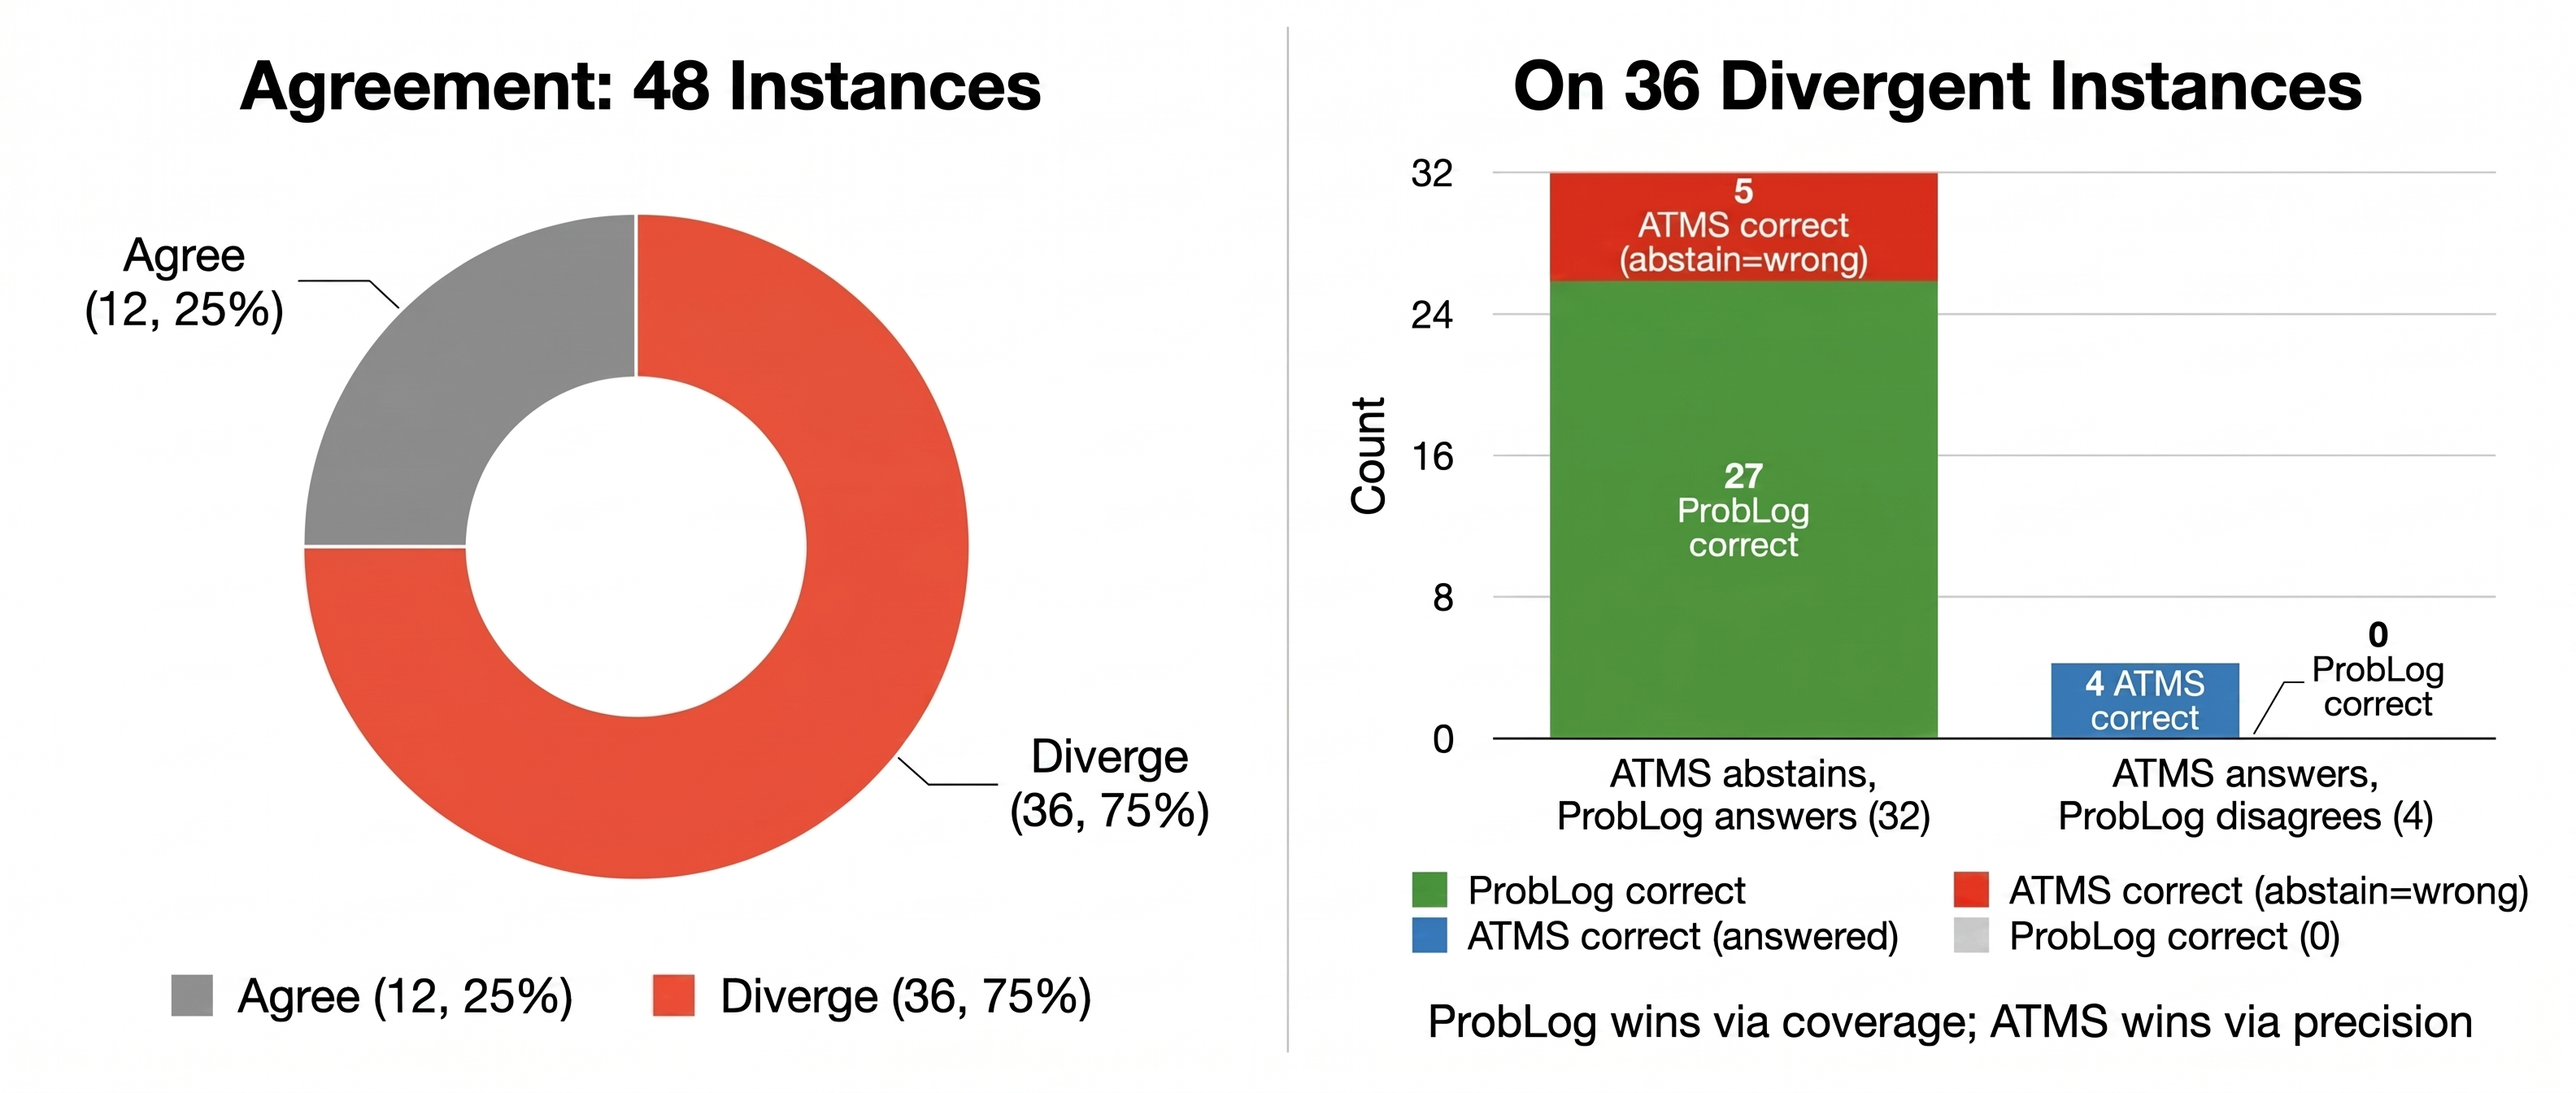
\includegraphics[width=\textwidth,height=0.45\textheight,keepaspectratio]{figures/fig4_v0.jpg}
  \caption{On 36 of 48 instances (75\%) where ATMS and ProbLog disagree, ProbLog is correct on 30
  (83.3\%) and ATMS on 6 (16.7\%). The divergence arises primarily because ATMS abstains
  ($\lambda=\infty$) while ProbLog commits to an answer using independent Bernoulli probabilities. On
  the 4 instances where ATMS affirmatively answers and ProbLog disagrees, ATMS wins all 4.}
  \label{fig:divergence}
\end{figure*}

\subsection{Ablations}

\noindent\textbf{Assumption threshold sensitivity.} At $\theta=0$ (answer only empty-environment
conclusions), coverage drops to 20.8\% (10/48) and accuracy reaches 90.0\% on answered instances. At
$\theta=2$, coverage is 22.9\% with 90.9\% accuracy. The threshold provides a direct
coverage--precision knob requiring no labels.

\noindent\textbf{Assumption-load vs.\ LLM confidence as abstention signals.} AUROC for assumption-load
as a binary error predictor is 0.777; for LLM verbalized confidence, AUROC is approximately 0.40.
Assumption-load substantially outperforms LLM verbalized confidence as an abstention signal on this
dataset.

\noindent\textbf{70B model ablation.} The 70B model ablation (\texttt{meta-llama/llama-3.1-70b-instruct})
was planned but not executed due to budget constraints in iter-2; the abstain rate on that run was
already 96.7\% with the 8B model, and larger-model results would require a separate evaluation. This
remains a key open question: whether a more capable model can propose richer assumption sets that yield
bounded derivations for a higher fraction of documents.

\section{Discussion}

\subsection{Interpretation of Results}

The primary mechanism driving the ATMS's selective precision is \textbf{conservative binary abstention}:
when the bounded ATMS finds no consistent derivation within depth $d=3$, it emits $\lambda=\infty$ and
abstains. This produces a bimodal distribution---a small high-precision answered set and a large
abstained set---rather than the graduated confidence scores assumed by the H2 monotonicity hypothesis.
The strong Spearman correlation ($\rho=0.629$) reflects this bimodal structure: $\lambda=0$ instances
are 90\% correct, $\lambda=\infty$ instances are 19\% correct.

The practical contribution is strongest in \textbf{precision-critical settings} where abstention is
preferable to hallucination (legal document review, medical diagnosis, compliance checking). In
coverage-critical settings, the 77.1\% abstain rate is prohibitive unless paired with a fallback
policy.

The ATMS--ProbLog divergence result clarifies an important distinction: ATMS abstention is the
conservative choice on correlated assumptions, while ProbLog's independence assumption allows it to
commit to an answer. On this evaluation, ProbLog's willingness to commit wins 30 of 36 divergent
cases. This does not mean ProbLog is better in general---the independence assumption is formally
incorrect for correlated assumptions---but it does mean ATMS's structural correctness comes at a
coverage cost that practitioners must account for.

\subsection{Related Work}

LINC~\citep{Olausson2023} explores the ambiguity space by voting over $K$ independently-sampled
whole-translations. This unstructured sampling cannot localize which choice drove the result, and on
this evaluation, LINC-calibrated abstention (at 22.9\% coverage) yields 72.7\% accuracy, below the
ATMS's 90.9\%. Logic-LM~\citep{Pan2023} self-refines a single formalization using solver syntax
errors; it cannot represent competing semantic completions or produce per-conclusion risk scores.
Path-of-Thoughts~\citep{Zhang2024} confirms, with its 95.9\% triplet-extraction accuracy, that L1
grounding error is a real and measurable channel---exactly what our two-layer architecture quantifies.

VeriCoT~\citep{Feng2025} validates single-theory steps with a solver, producing binary verdicts with
no per-conclusion risk score. ALP counter-abduction~\citep{Galitsky2026} operates on and repairs a
single completed explanation; it does not maintain competing completions as parallel tracked
assumptions and produces no assumption-load lattice.

Conformal abstention~\citep{AbbasiYadkori2024} achieves distribution-free coverage guarantees but
requires a labeled calibration set; our criterion needs no labels and gives conclusion-specific
structural control. Imprecise-probability methods~\citep{Yang2026} elicit uncertainty as intervals
directly from the LLM; we derive uncertainty structurally from explicit choice-points, so
empty-environment conclusions are certified independent of LLM calibration.
Hypotheses-to-Theories~\citep{Zhu2023} induces a global rule library on labeled training examples; we
need no labels and no training set, proposing and tracking assumptions per-document at inference time.

De~Kleer's original ATMS~\citep{deKleer1986} and his incremental prime-implicate
algorithm~\citep{deKleer1992} are the imported mechanism; to our knowledge no prior work maps LLM
formalization under-determinacy onto ATMS assumptions or uses empty-environment derivability as a
hallucination criterion.

\subsection{Limitations}

The evaluation is underpowered. H1 (empty-env precision = 90\%) rests on $n=10$; the 95\% CI spans
59.6\%--98.2\%. H2 is supported on $n=48$ but the stratum structure ($n=1$ for load=1) prevents
per-stratum trend testing. A scaled evaluation of at least 500 instances with at least 50
empty-environment derivable conclusions is required for definitive claims.

The 77.1\% abstain rate is the dominant practical limitation. On the harder RuleTaker/ProofWriter
benchmark, this rises to 96.7\%, effectively making the method inapplicable. The 8B model's limited
ability to generate coherent assumption-set proposals is the likely proximate cause; the 70B ablation
was not executed and remains an open question.

The bounded ATMS (depth cap $d=3$, beam width $b=20$) was never activated in these evaluations: exact
ATMS sufficed because mean choice points (2.4--3.5) were well below the threshold. The bounded
approximation's accuracy under denser assumption graphs is uncharacterized.

Logic-LM and ALP counter-abduction are compared qualitatively; quantitative comparison on the same
instances is deferred to future work.

\section{Conclusion}

We presented the Empty-Environment Test: a two-layer neuro-symbolic pipeline that imports de~Kleer's
ATMS, in a tractability-bounded form, to separate L1 grounding error from L2 assumption error in
text-to-logic reasoning. The corrected evaluation shows assumption-load is a strong, significant error
predictor ($\rho=0.629$, $p<0.001$, AUROC $=0.777$). At 22.9\% coverage, the method achieves 90.9\%
accuracy, exceeding CoT (72.7\%) and LINC (72.7\%) at matched coverage. Empty-environment conclusions
reach 90\% precision with zero label supervision; the L1 degradation bound gives a non-trivial floor
of 0.885 at realistic grounding error rates.

The key limitation is conservative: a 77.1\% abstain rate makes the method applicable primarily to
precision-critical settings. Future work should evaluate with larger models to reduce abstention, scale
to 500+ instances to establish statistical power, and test the bounded approximation on denser document
sets.

Reframing hallucination as a structural property of logical support---rather than a property of
generated text---is the mechanism, not just an analogy. The cross-domain transfer from classical
model-based diagnosis to modern LLM governance provides the specific algorithmic tool: an environment
lattice that certifies which conclusions the document forces, which depend on unverified choices, and
which cannot be derived at all.

\bibliography{references}
\bibliographystyle{plainnat}

\end{document}
